% Created by tikzDevice version 0.12.4 on 2023-07-06 13:18:37
% !TEX encoding = UTF-8 Unicode
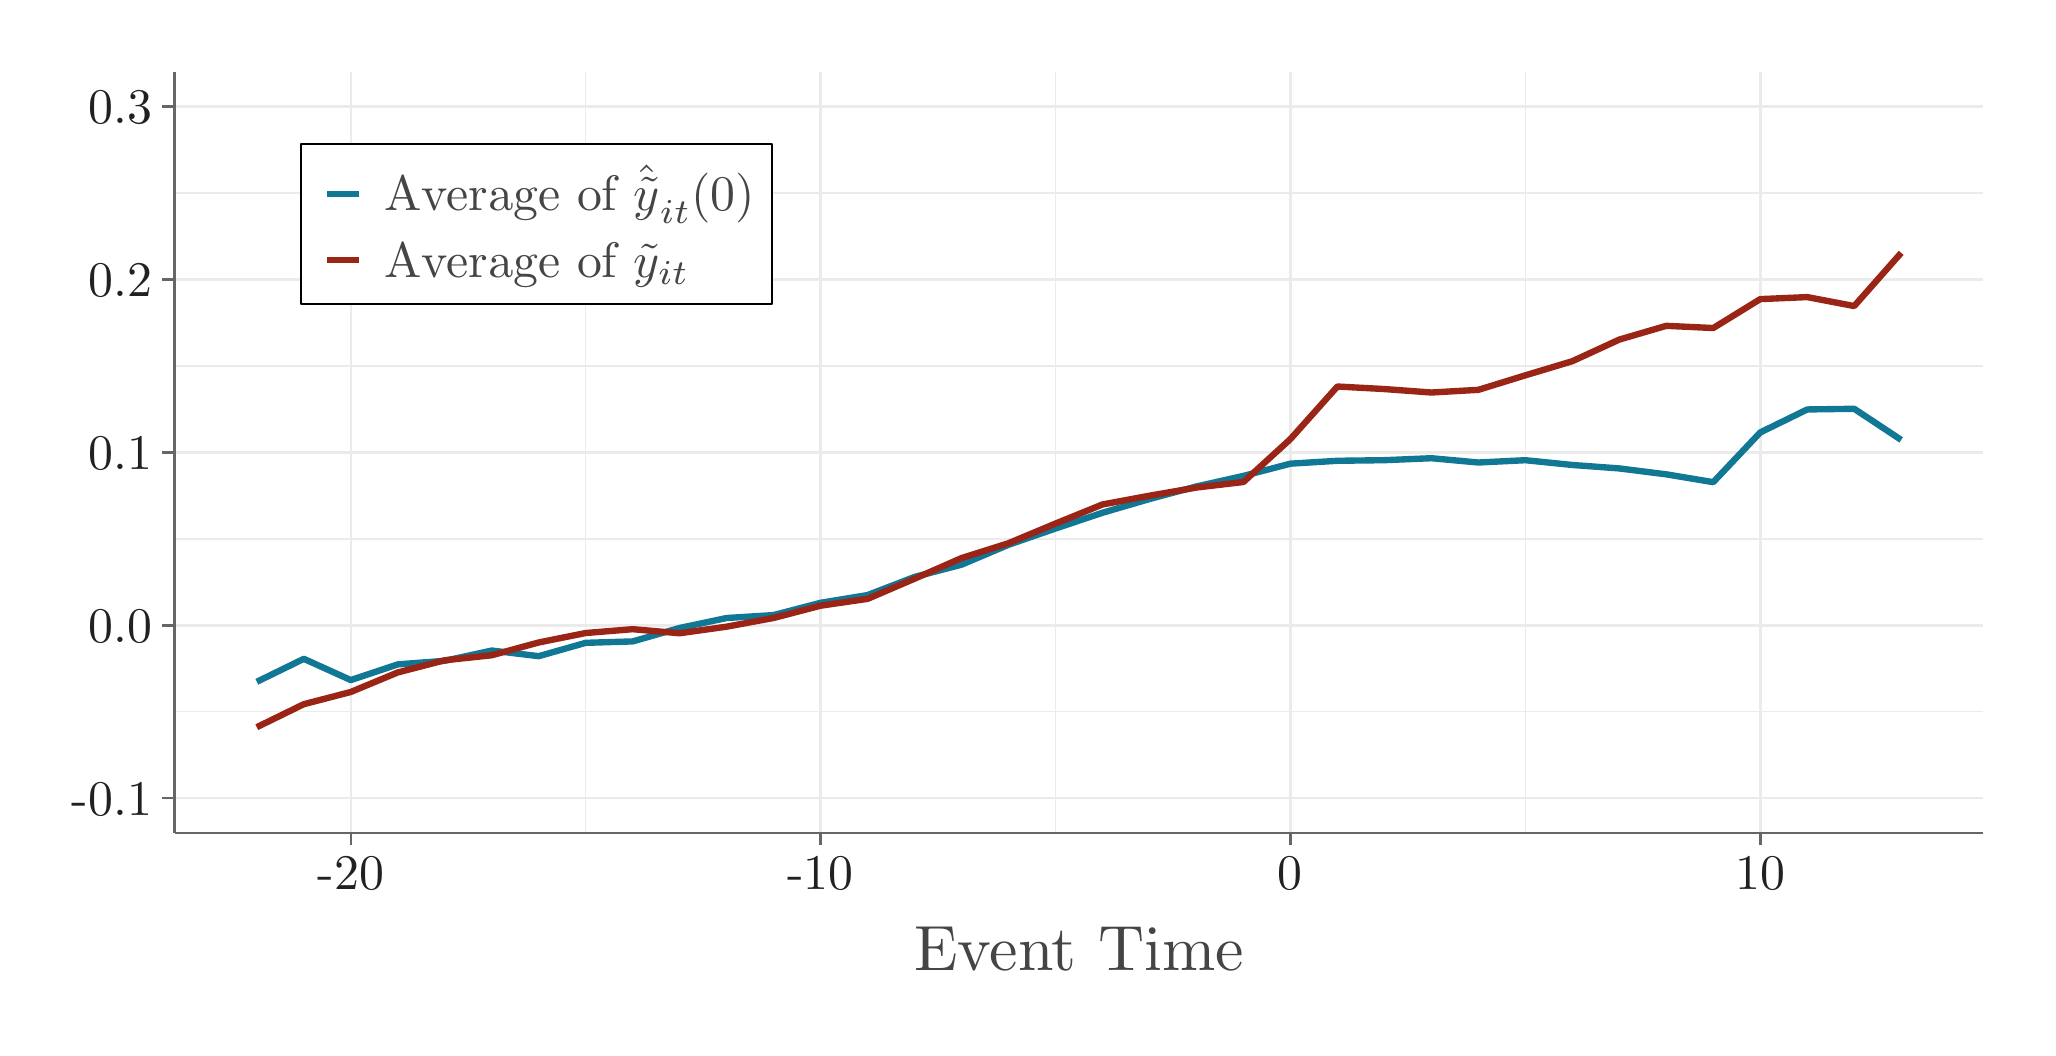
\begin{tikzpicture}[x=1pt,y=1pt]
\definecolor{fillColor}{RGB}{255,255,255}
\path[use as bounding box,fill=fillColor,fill opacity=0.00] (0,0) rectangle (722.70,361.35);
\begin{scope}
\path[clip] (  0.00,  0.00) rectangle (722.70,361.35);
\definecolor{fillColor}{RGB}{255,255,255}

\path[fill=fillColor] (  0.00, -0.00) rectangle (722.70,361.35);
\end{scope}
\begin{scope}
\path[clip] ( 53.09, 70.42) rectangle (706.70,345.35);
\definecolor{fillColor}{RGB}{255,255,255}

\path[fill=fillColor] ( 53.09, 70.42) rectangle (706.70,345.35);
\definecolor{drawColor}{gray}{0.92}

\path[draw=drawColor,line width= 0.5pt,line join=round] ( 53.09,114.16) --
	(706.70,114.16);

\path[draw=drawColor,line width= 0.5pt,line join=round] ( 53.09,176.64) --
	(706.70,176.64);

\path[draw=drawColor,line width= 0.5pt,line join=round] ( 53.09,239.13) --
	(706.70,239.13);

\path[draw=drawColor,line width= 0.5pt,line join=round] ( 53.09,301.61) --
	(706.70,301.61);

\path[draw=drawColor,line width= 0.5pt,line join=round] (201.64, 70.42) --
	(201.64,345.35);

\path[draw=drawColor,line width= 0.5pt,line join=round] (371.41, 70.42) --
	(371.41,345.35);

\path[draw=drawColor,line width= 0.5pt,line join=round] (541.18, 70.42) --
	(541.18,345.35);

\path[draw=drawColor,line width= 0.9pt,line join=round] ( 53.09, 82.92) --
	(706.70, 82.92);

\path[draw=drawColor,line width= 0.9pt,line join=round] ( 53.09,145.40) --
	(706.70,145.40);

\path[draw=drawColor,line width= 0.9pt,line join=round] ( 53.09,207.89) --
	(706.70,207.89);

\path[draw=drawColor,line width= 0.9pt,line join=round] ( 53.09,270.37) --
	(706.70,270.37);

\path[draw=drawColor,line width= 0.9pt,line join=round] ( 53.09,332.85) --
	(706.70,332.85);

\path[draw=drawColor,line width= 0.9pt,line join=round] (116.76, 70.42) --
	(116.76,345.35);

\path[draw=drawColor,line width= 0.9pt,line join=round] (286.52, 70.42) --
	(286.52,345.35);

\path[draw=drawColor,line width= 0.9pt,line join=round] (456.29, 70.42) --
	(456.29,345.35);

\path[draw=drawColor,line width= 0.9pt,line join=round] (626.06, 70.42) --
	(626.06,345.35);
\definecolor{drawColor}{RGB}{16,120,149}

\path[draw=drawColor,line width= 2.3pt,line join=round] ( 82.80,124.98) --
	( 99.78,133.28) --
	(116.76,125.61) --
	(133.73,131.27) --
	(150.71,132.57) --
	(167.69,136.27) --
	(184.66,134.24) --
	(201.64,139.06) --
	(218.62,139.57) --
	(235.59,144.43) --
	(252.57,148.03) --
	(269.55,149.09) --
	(286.52,153.53) --
	(303.50,156.32) --
	(320.48,162.87) --
	(337.45,167.30) --
	(354.43,174.49) --
	(371.41,180.37) --
	(388.38,186.06) --
	(405.36,191.02) --
	(422.34,195.57) --
	(439.32,199.38) --
	(456.29,203.80) --
	(473.27,204.84) --
	(490.25,205.06) --
	(507.22,205.77) --
	(524.20,204.22) --
	(541.18,205.05) --
	(558.15,203.33) --
	(575.13,202.08) --
	(592.11,199.94) --
	(609.08,197.12) --
	(626.06,215.08) --
	(643.04,223.39) --
	(660.01,223.63) --
	(676.99,212.39);
\definecolor{drawColor}{RGB}{154,36,21}

\path[draw=drawColor,line width= 2.3pt,line join=round] ( 82.80,108.58) --
	( 99.78,116.89) --
	(116.76,121.30) --
	(133.73,128.36) --
	(150.71,132.76) --
	(167.69,134.57) --
	(184.66,139.19) --
	(201.64,142.61) --
	(218.62,143.99) --
	(235.59,142.52) --
	(252.57,144.90) --
	(269.55,148.04) --
	(286.52,152.48) --
	(303.50,154.95) --
	(320.48,162.23) --
	(337.45,169.69) --
	(354.43,175.06) --
	(371.41,182.16) --
	(388.38,189.06) --
	(405.36,192.22) --
	(422.34,195.17) --
	(439.32,197.18) --
	(456.29,212.69) --
	(473.27,231.68) --
	(490.25,230.76) --
	(507.22,229.51) --
	(524.20,230.48) --
	(541.18,235.72) --
	(558.15,240.82) --
	(575.13,248.64) --
	(592.11,253.61) --
	(609.08,252.81) --
	(626.06,263.26) --
	(643.04,263.99) --
	(660.01,260.75) --
	(676.99,279.97);

\path[] ( 53.09, 70.42) rectangle (706.70,345.35);
\end{scope}
\begin{scope}
\path[clip] (  0.00,  0.00) rectangle (722.70,361.35);
\definecolor{drawColor}{gray}{0.40}

\path[draw=drawColor,line width= 0.9pt,line join=round] ( 53.09, 70.42) --
	( 53.09,345.35);
\end{scope}
\begin{scope}
\path[clip] (  0.00,  0.00) rectangle (722.70,361.35);
\definecolor{drawColor}{gray}{0.13}

\node[text=drawColor,anchor=base east,inner sep=0pt, outer sep=0pt, scale=  1.80] at ( 44.99, 76.72) {-0.1};

\node[text=drawColor,anchor=base east,inner sep=0pt, outer sep=0pt, scale=  1.80] at ( 44.99,139.20) {0.0};

\node[text=drawColor,anchor=base east,inner sep=0pt, outer sep=0pt, scale=  1.80] at ( 44.99,201.69) {0.1};

\node[text=drawColor,anchor=base east,inner sep=0pt, outer sep=0pt, scale=  1.80] at ( 44.99,264.17) {0.2};

\node[text=drawColor,anchor=base east,inner sep=0pt, outer sep=0pt, scale=  1.80] at ( 44.99,326.65) {0.3};
\end{scope}
\begin{scope}
\path[clip] (  0.00,  0.00) rectangle (722.70,361.35);
\definecolor{drawColor}{gray}{0.40}

\path[draw=drawColor,line width= 0.9pt,line join=round] ( 48.59, 82.92) --
	( 53.09, 82.92);

\path[draw=drawColor,line width= 0.9pt,line join=round] ( 48.59,145.40) --
	( 53.09,145.40);

\path[draw=drawColor,line width= 0.9pt,line join=round] ( 48.59,207.89) --
	( 53.09,207.89);

\path[draw=drawColor,line width= 0.9pt,line join=round] ( 48.59,270.37) --
	( 53.09,270.37);

\path[draw=drawColor,line width= 0.9pt,line join=round] ( 48.59,332.85) --
	( 53.09,332.85);
\end{scope}
\begin{scope}
\path[clip] (  0.00,  0.00) rectangle (722.70,361.35);
\definecolor{drawColor}{gray}{0.40}

\path[draw=drawColor,line width= 0.9pt,line join=round] ( 53.09, 70.42) --
	(706.70, 70.42);
\end{scope}
\begin{scope}
\path[clip] (  0.00,  0.00) rectangle (722.70,361.35);
\definecolor{drawColor}{gray}{0.40}

\path[draw=drawColor,line width= 0.9pt,line join=round] (116.76, 65.92) --
	(116.76, 70.42);

\path[draw=drawColor,line width= 0.9pt,line join=round] (286.52, 65.92) --
	(286.52, 70.42);

\path[draw=drawColor,line width= 0.9pt,line join=round] (456.29, 65.92) --
	(456.29, 70.42);

\path[draw=drawColor,line width= 0.9pt,line join=round] (626.06, 65.92) --
	(626.06, 70.42);
\end{scope}
\begin{scope}
\path[clip] (  0.00,  0.00) rectangle (722.70,361.35);
\definecolor{drawColor}{gray}{0.13}

\node[text=drawColor,anchor=base,inner sep=0pt, outer sep=0pt, scale=  1.80] at (116.76, 49.93) {-20};

\node[text=drawColor,anchor=base,inner sep=0pt, outer sep=0pt, scale=  1.80] at (286.52, 49.93) {-10};

\node[text=drawColor,anchor=base,inner sep=0pt, outer sep=0pt, scale=  1.80] at (456.29, 49.93) {0};

\node[text=drawColor,anchor=base,inner sep=0pt, outer sep=0pt, scale=  1.80] at (626.06, 49.93) {10};
\end{scope}
\begin{scope}
\path[clip] (  0.00,  0.00) rectangle (722.70,361.35);
\definecolor{drawColor}{gray}{0.27}

\node[text=drawColor,anchor=base,inner sep=0pt, outer sep=0pt, scale=  2.31] at (379.90, 20.50) {Event Time};
\end{scope}
\begin{scope}
\path[clip] (  0.00,  0.00) rectangle (722.70,361.35);
\definecolor{drawColor}{RGB}{0,0,0}
\definecolor{fillColor}{RGB}{255,255,255}

\path[draw=drawColor,line width= 0.6pt,line join=round,line cap=round,fill=fillColor] ( 98.75,261.47) rectangle (268.88,319.26);
\end{scope}
\begin{scope}
\path[clip] (  0.00,  0.00) rectangle (722.70,361.35);
\definecolor{fillColor}{RGB}{255,255,255}

\path[fill=fillColor] (106.75,293.36) rectangle (121.21,309.26);
\end{scope}
\begin{scope}
\path[clip] (  0.00,  0.00) rectangle (722.70,361.35);
\definecolor{drawColor}{RGB}{16,120,149}

\path[draw=drawColor,line width= 2.3pt,line join=round] (108.20,301.31) -- (119.76,301.31);
\end{scope}
\begin{scope}
\path[clip] (  0.00,  0.00) rectangle (722.70,361.35);
\definecolor{fillColor}{RGB}{255,255,255}

\path[fill=fillColor] (106.75,269.47) rectangle (121.21,285.36);
\end{scope}
\begin{scope}
\path[clip] (  0.00,  0.00) rectangle (722.70,361.35);
\definecolor{drawColor}{RGB}{154,36,21}

\path[draw=drawColor,line width= 2.3pt,line join=round] (108.20,277.42) -- (119.76,277.42);
\end{scope}
\begin{scope}
\path[clip] (  0.00,  0.00) rectangle (722.70,361.35);
\definecolor{drawColor}{gray}{0.27}

\node[text=drawColor,anchor=base west,inner sep=0pt, outer sep=0pt, scale=  1.80] at (128.95,295.11) {Average of $\hat{\tilde{y}}_{it}(0)$};
\end{scope}
\begin{scope}
\path[clip] (  0.00,  0.00) rectangle (722.70,361.35);
\definecolor{drawColor}{gray}{0.27}

\node[text=drawColor,anchor=base west,inner sep=0pt, outer sep=0pt, scale=  1.80] at (128.95,271.22) {Average of $\tilde{y}_{it}$};
\end{scope}
\end{tikzpicture}
